\documentclass[11pt,a4paper]{article}

\usepackage[utf8]{inputenc}
\usepackage[T1]{fontenc}
\usepackage{mathpazo}
\usepackage[scaled=0.92]{helvet}
\usepackage[margin=1in]{geometry}
\usepackage{graphicx}
\usepackage{amsmath,amssymb,amsfonts}
\usepackage{booktabs}
\usepackage{tabularx}
\usepackage{setspace}
\usepackage{titlesec}
\usepackage{fancyhdr}
\usepackage{float}
\usepackage{caption}
\usepackage{microtype}
\usepackage{tikz}
\usepackage{xcolor}
\usepackage[hidelinks]{hyperref}

\usetikzlibrary{shapes.geometric, arrows.meta, positioning, calc, matrix, fit, backgrounds}

\setstretch{1.15}
\setlength{\parindent}{0pt}
\setlength{\parskip}{0.8em}
\sloppy

\titleformat{\section}{\normalfont\large\bfseries\sffamily}{\thesection}{1em}{}
\titleformat{\subsection}{\normalfont\normalsize\bfseries\sffamily}{\thesubsection}{1em}{}
\titleformat{\subsubsection}{\normalfont\normalsize\itshape\sffamily}{\thesubsubsection}{1em}{}

\pagestyle{fancy}
\fancyhf{}
\fancyhead[L]{\small\sffamily Content-Addressable Storage}
\fancyhead[R]{\small\sffamily\thepage}
\renewcommand{\headrulewidth}{0.4pt}

\captionsetup{font=small,labelfont=bf,labelsep=period}

\renewenvironment{abstract}
{\small
	\begin{center}\textbf{\sffamily Abstrak}\end{center}
	\begin{quote}}
	{\end{quote}}

\lstdefinestyle{code}{
	basicstyle=\ttfamily\small,
	frame=single,
	rulecolor=\color{black},
	breaklines=true,
	showstringspaces=false,
	columns=fullflexible,
	keepspaces=true,
	framesep=6pt,
	aboveskip=1em,
	belowskip=1em,
	xleftmargin=0pt
}

\lstdefinestyle{out}{
	basicstyle=\ttfamily\small,
	frame=tb,
	rulecolor=\color{black},
	breaklines=true,
	showstringspaces=false,
	columns=fullflexible,
	keepspaces=true,
	framesep=4pt,
	aboveskip=1em,
	belowskip=1em
}

\title{\vspace{-1.5cm}\textbf{\sffamily\LARGE Content-Addressable Storage\\ Fondasi Penyimpanan pada Sistem Kontrol Versi}}
\author{
	\textbf{Muhammad Riduwan Khafidi} \\
	\small Program Studi Teknik Rekayasa Perangkat Lunak \\
	\small Politeknik Negeri Batam \\
	\small \texttt{4342611034@students.polibatam.ac.id}
}
\date{\small\today}

\begin{document}

\maketitle
\thispagestyle{empty}

\begin{abstract}
	Content-addressable storage adalah model penyimpanan di mana alamat setiap objek ditentukan oleh isi objek itu sendiri, bukan oleh lokasi fisik atau nomor urut. Model ini menjadi fondasi Git, Mercurial, dan sistem kontrol versi modern karena memungkinkan deduplikasi otomatis, immutability, dan verifikasi integritas bawaan. Makalah ini membedah mekanisme content-addressable storage dalam sistem kontrol versi dari empat perspektif: hash sebagai alamat, empat tipe objek dasar, struktur Merkle yang menjamin immutability, serta siklus hidup satu commit dari pembuatan hingga penyimpanan. Setiap perspektif dilengkapi analogi konkret, contoh berangka, dan sembilan visualisasi TikZ yang menyoroti hubungan antar komponen. Melalui kerangka ini, pembaca memperoleh mental model untuk membaca implementasi VCS mana pun, dari Git hingga sistem kustom seperti libvctrl.
\end{abstract}

\section{Pendahuluan}

\subsection{Analogi Pembuka}

Bayangkan sebuah perpustakaan di mana setiap buku tidak diberi nomor rak, tidak diberi kode katalog, dan tidak diberi label tanggal masuk. Setiap buku justru diidentifikasi oleh isinya sendiri: judul, penulis, dan seluruh teksnya diolah menjadi sidik jari unik. Jika dua buku identik datang, pustakawan tidak menyimpan dua salinan; ia menyimpan satu, karena keduanya memiliki sidik jari yang sama. Jika isi sebuah buku berubah sedikit saja, sidik jarinya berubah total, sehingga buku lama dan buku baru menempati alamat yang berbeda.

Perpustakaan itu adalah content-addressable storage. Setiap buku adalah objek. Sidik jari adalah hash kriptografis. Alamatnya bukan nomor urut, melainkan hash dari isi. Sistem kontrol versi modern seperti Git dan libvctrl menggunakan model ini untuk menyimpan seluruh riwayat proyek: setiap file, setiap direktori, dan setiap commit memiliki alamat yang ditentukan oleh isinya, bukan oleh kapan atau di mana ia disimpan.

\subsection{Mengapa Topik Ini Penting}

Seorang pengembang yang memahami content-addressable storage dapat menjelaskan mengapa Git tidak menggandakan file saat berpindah branch, mengapa commit yang isinya sama selalu memiliki hash yang sama, dan mengapa sebuah file yang sudah dihapus dari working directory tetap ada di riwayat selama masih dirujuk oleh commit. Tanpa pemahaman ini, pengembang cenderung memperlakukan Git sebagai kotak hitam, memakai perintah tanpa mengerti biaya dan jaminan yang melekat padanya.

Selain itu, model ini adalah jawaban paling bersih untuk dua masalah lama dalam penyimpanan data: deduplikasi dan integritas. Sistem berkas konvensional menyimpan dua file identik sebagai dua salinan, dan tidak memiliki cara bawaan untuk mendeteksi korupsi. Content-addressable storage menyimpan satu salinan untuk setiap isi unik, dan mendeteksi korupsi secara otomatis karena hash dari isi yang rusak tidak akan cocok dengan alamat yang tercatat.

\subsection{Peta Pembahasan}

Makalah ini dibagi menjadi empat bagian konsep. Bagian kedua membahas hash sebagai alamat, termasuk properti kriptografis yang membuatnya layak dipercaya. Bagian ketiga membahas empat tipe objek dasar pada object store: \texttt{blob}, \texttt{tree}, \texttt{commit}, dan \texttt{tag}. Bagian keempat membahas struktur Merkle yang menghubungkan objek-objek tersebut dan immutability sebagai sifat bawaan. Bagian kelima menyandingkan model content-addressable dengan model address-based konvensional. Bagian keenam membawa seluruh konsep ke studi kasus delapan langkah menyimpan satu commit dari nol. Bagian ketujuh dan kedelapan merangkum kesalahan umum dan lembar rujukan cepat. Bagian kesembilan menutup dengan tiga prinsip.

\section{Hash sebagai Alamat Konten}

\subsection{Definisi dan Analogi}

Hash kriptografis adalah fungsi yang menerima input dengan panjang berapa pun dan menghasilkan output dengan panjang tetap, dengan jaminan bahwa input yang berbeda menghasilkan output yang berbeda hampir sepanjang waktu. Pada content-addressable storage, output inilah yang menjadi alamat.

Analogi paling dekat adalah cap jari manusia. Dua orang bisa memiliki nama yang sama, tetapi tidak bisa memiliki cap jari yang sama. Nama adalah alamat yang bisa bertabrakan; cap jari adalah alamat yang hampir tidak mungkin bertabrakan. Content-addressable storage memakai cap jari, bukan nama.

\subsection{Mengapa Hash, Bukan Nomor Urut}

Sistem berkas konvensional memberi alamat pada file berdasarkan nomor inode, path, atau offset. Alamat itu stabil selama file tidak dipindahkan, tetapi tidak memberi informasi apa pun tentang isi. Sistem kontrol versi membutuhkan tiga hal yang tidak bisa diberikan oleh alamat konvensional.

Pertama, deduplikasi. Jika dua commit menyimpan file yang identik, sistem tidak perlu menyimpannya dua kali. Dengan alamat berbasis isi, keduanya memiliki alamat yang sama, dan penyimpanan kedua tidak melakukan apa-apa.

Kedua, verifikasi integritas. Jika file di disk rusak, sistem bisa menghitung ulang hash dan membandingkannya dengan alamat. Ketidakcocokan menandakan korupsi. Model address-based tidak memiliki cara ini.

Ketiga, immutability. Objek yang alamatnya ditentukan oleh isi tidak bisa diubah tanpa mengubah alamatnya. Sistem bisa mengasumsikan bahwa objek dengan alamat tertentu selalu memiliki isi yang sama, di mana pun dan kapan pun.

Gambar~\ref{fig:address-vs-content} menyandingkan kedua model.

\begin{figure}[H]
	\centering
	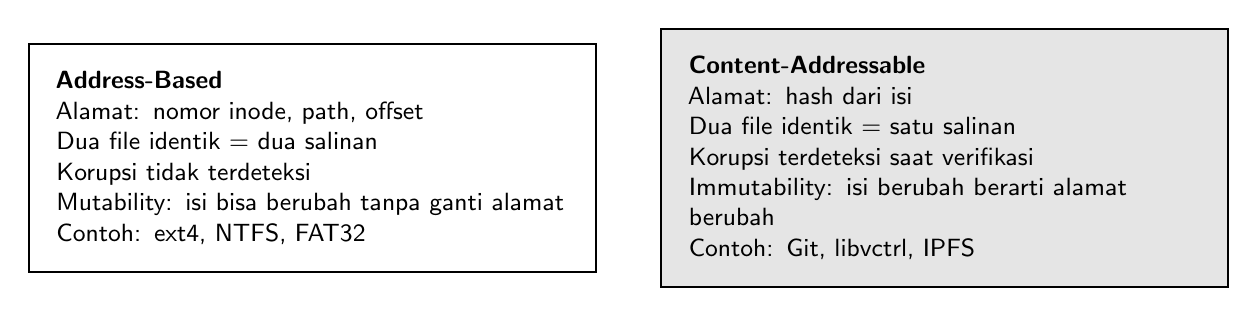
\begin{tikzpicture}[
			box/.style={rectangle, draw=black, thick, text width=6.5cm, align=left, font=\sffamily\small, inner sep=10pt}
		]
		\node[box, fill=white] (a) {
			\textbf{Address-Based} \\
			Alamat: nomor inode, path, offset \\
			Dua file identik = dua salinan \\
			Korupsi tidak terdeteksi \\
			Mutability: isi bisa berubah tanpa ganti alamat \\
			Contoh: ext4, NTFS, FAT32
		};
		\node[box, fill=black!10, right=0.8cm of a] (b) {
			\textbf{Content-Addressable} \\
			Alamat: hash dari isi \\
			Dua file identik = satu salinan \\
			Korupsi terdeteksi saat verifikasi \\
			Immutability: isi berubah berarti alamat berubah \\
			Contoh: Git, libvctrl, IPFS
		};
	\end{tikzpicture}
	\caption{Perbandingan alamat berbasis posisi dengan alamat berbasis konten.}
	\label{fig:address-vs-content}
\end{figure}

\subsection{Properti Kriptografis yang Wajib Dipenuhi}

Tidak semua fungsi hash layak menjadi alamat. Ada tiga properti yang wajib dipenuhi.

Pertama, determinisme. Input yang sama harus selalu menghasilkan output yang sama. Jika hash bisa berubah antar pemanggilan, alamat tidak lagi stabil, dan seluruh model runtuh.

Kedua, ketahanan tabrakan. Dua input berbeda harus menghasilkan output yang berbeda, kecuali dengan probabilitas yang sangat kecil. Untuk SHA-256, probabilitas tabrakan acak sekitar satu banding dua pangkat seratus dua puluh delapan. Angka ini jauh lebih kecil daripada probabilitas hard disk gagal secara fisik pada saat yang sama.

Ketiga, ketahanan preimage. Dari hash, tidak mungkin menghitung input aslinya dalam waktu yang wajar. Sifat ini melindungi objek dari pemalsuan: penyerang tidak bisa membuat objek dengan hash tertentu tanpa memiliki isi yang sesuai.

Ketiga properti ini adalah alasan mengapa SHA-256 dan SHA-512 dipakai, bukan fungsi hash non-kriptografis seperti CRC32 atau MD5 (yang sudah dianggap rusak untuk keperluan ini). Tabel~\ref{tab:hash-props} merangkumnya.

\begin{table}[H]
	\centering
	\caption{Properti kriptografis yang wajib dimiliki fungsi hash alamat.}
	\label{tab:hash-props}
	\small
	\begin{tabularx}{\textwidth}{l X X}
		\toprule
		Properti            & Arti                                & Akibat jika gagal                       \\
		\midrule
		Deterministik       & input sama, output sama             & alamat tidak stabil, tidak bisa dipakai \\
		Collision-resistant & input beda, output beda             & dua objek bisa bertabrakan alamatnya    \\
		Avalanche           & ubah satu bit, output berubah total & perubahan kecil tidak terdeteksi        \\
		Preimage-resistant  & tidak bisa balik dari hash ke input & objek bisa dipalsukan                   \\
		\bottomrule
	\end{tabularx}
\end{table}

\subsection{Contoh Berangka}

Mari hitung hash dari dua string yang berbeda satu karakter. Perintahnya memakai \texttt{sha256sum} yang universal.

\begin{lstlisting}[style=code]
echo -n "hello" | sha256sum
echo -n "hellp" | sha256sum
\end{lstlisting}

Keluaran kedua perintah:

\begin{lstlisting}[style=out]
2cf24dba5fb0a30e26e83b2ac5b9e29e1b161e5c1fa7425e73043362938b9824  -
ea09ae9cc6768c50fcee903ed054556e5bfc8347907f12598aa241203221d2b0  -
\end{lstlisting}

Dua input yang berbeda satu karakter menghasilkan dua hash yang sama sekali berbeda. Inilah yang disebut efek avalanche: perubahan kecil menyebar ke seluruh output. Untuk content-addressable storage, sifat ini berarti bahwa setiap perubahan pada file menghasilkan alamat baru, sehingga versi lama tetap bisa diakses melalui alamat lamanya.

\section{Object Store: Empat Tipe Dasar}

\subsection{Mengapa Empat Tipe, Bukan Satu}

Jika seluruh data disimpan sebagai byte stream tanpa tipe, sistem tidak bisa membedakan file dari direktori, atau direktori dari commit. Setiap operasi harus menebak tipe dari isinya, yang lambat dan rawan salah. Object store modern memecah data menjadi empat tipe yang masing-masing memiliki peran jelas: \texttt{blob}, \texttt{tree}, \texttt{commit}, dan \texttt{tag}. Gambar~\ref{fig:object-types} menunjukkan hierarkinya.

\begin{figure}[H]
	\centering
	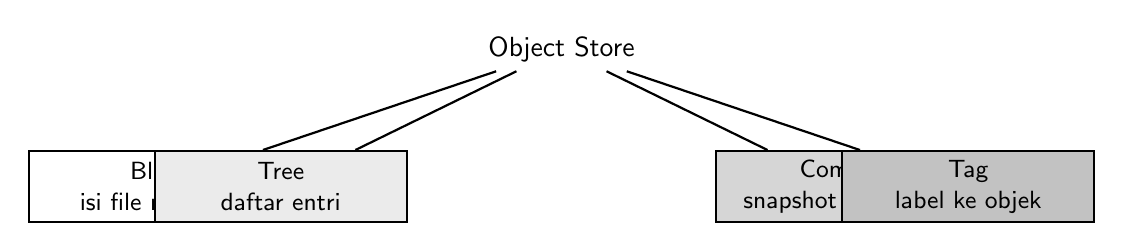
\begin{tikzpicture}[
			node distance=0.5cm and 0.8cm,
			cat/.style={rectangle, draw=black, thick, fill=white, minimum width=3.2cm, minimum height=0.9cm, align=center, font=\sffamily\small},
			line/.style={draw, thick}
		]
		\node[font=\sffamily] (root) at (0, 1) {Object Store};
		\node[cat, fill=white, below left=1cm and 2.5cm of root] (blob) {Blob \\ isi file mentah};
		\node[cat, fill=black!8, below left=1cm and 0.9cm of root] (tree) {Tree \\ daftar entri};
		\node[cat, fill=black!16, below right=1cm and 0.9cm of root] (commit) {Commit \\ snapshot + parent};
		\node[cat, fill=black!24, below right=1cm and 2.5cm of root] (tag) {Tag \\ label ke objek};

		\draw[line] (root) -- (blob);
		\draw[line] (root) -- (tree);
		\draw[line] (root) -- (commit);
		\draw[line] (root) -- (tag);
	\end{tikzpicture}
	\caption{Empat tipe objek pada content-addressable object store.}
	\label{fig:object-types}
\end{figure}

\subsection{Blob: Isi File Mentah}

\texttt{blob} adalah singkatan dari \textit{binary large object}. Isinya adalah byte mentah dari sebuah file, tanpa nama, tanpa path, tanpa metadata apa pun. \texttt{blob} tidak tahu namanya sendiri; ia hanya tahu isinya.

Pemisahan nama dari isi ini adalah kunci deduplikasi. Jika file \texttt{notes.txt} dan \texttt{backup.txt} memiliki isi yang sama persis, keduanya merujuk ke \texttt{blob} yang sama. Sistem menyimpan satu \texttt{blob}, bukan dua.

Karena \texttt{blob} tidak menyimpan nama, cara sistem menemukan \texttt{blob} adalah melalui \texttt{tree}.

\subsection{Tree: Daftar Entri Direktori}

\texttt{tree} adalah satu tingkat direktori. Isinya adalah daftar entri, di mana setiap entri memiliki tiga komponen: nama, mode, dan hash dari objek target. Nama adalah nama file atau subdirektori. Mode adalah bit permission yang menyatakan apakah entri itu file biasa, file yang bisa dieksekusi, symlink, subdirektori, atau submodule. Hash adalah alamat dari \texttt{blob} (untuk file) atau \texttt{tree} (untuk subdirektori).

\texttt{tree} adalah tempat nama dan isi dipertemukan kembali. Sebuah \texttt{blob} bisa dirujuk oleh banyak \texttt{tree} dengan nama yang berbeda, dan sebuah \texttt{tree} bisa merujuk banyak \texttt{blob} dengan nama yang berbeda.

\subsection{Commit: Snapshot dengan Sejarah}

\texttt{commit} adalah snapshot dari seluruh \texttt{tree} di root proyek pada satu titik waktu, ditambah satu atau lebih \texttt{parent} yang menunjuk ke commit sebelumnya. Sebuah \texttt{commit} menyimpan hash dari root \texttt{tree}, daftar hash \texttt{parent}, penulis, committer, timestamp, pesan, dan metadata opsional seperti encoding.

Perbedaan antara \texttt{tree} dan \texttt{commit} adalah perbedaan antara "bagaimana isi direktori saat ini" dan "mengapa isi itu seperti ini". \texttt{tree} hanya menyimpan keadaan; \texttt{commit} menyimpan keadaan plus alasannya.

\subsection{Tag: Label yang Bisa Ditandatangani}

\texttt{tag} adalah label yang menunjuk ke objek lain, biasanya \texttt{commit}. Ada dua jenis: lightweight dan annotated. Lightweight hanyalah alias, sedangkan annotated adalah objek tersendiri yang menyimpan nama tag, hash target, tagger, pesan, dan tanda tangan kriptografis opsional.

Annotated \texttt{tag} adalah satu-satunya objek yang dirancang untuk ditandatangani. Tanda tangannya membuktikan bahwa tag itu dibuat oleh pemegang kunci privat, bukan oleh siapa pun yang bisa menulis ke repositori.

\subsection{Ringkasan Tipe Objek}

\begin{table}[H]
	\centering
	\caption{Ringkasan empat tipe objek pada object store.}
	\label{tab:object-types}
	\small
	\begin{tabularx}{\textwidth}{l X X}
		\toprule
		Tipe            & Isi utama                  & Peran                                   \\
		\midrule
		\texttt{blob}   & byte mentah dari satu file & menyimpan isi tanpa nama                \\
		\texttt{tree}   & daftar (nama, mode, hash)  & memetakan nama ke isi                   \\
		\texttt{commit} & tree + parent + metadata   & merekam snapshot dan sejarah            \\
		\texttt{tag}    & target + tagger + message  & label permanen yang bisa ditandatangani \\
		\bottomrule
	\end{tabularx}
\end{table}

\section{Struktur Merkle dan Immutability}

\subsection{Merkle: Hash dari Hash}

Setiap objek pada object store memiliki hash. Yang membuat struktur ini kuat adalah kenyataan bahwa \texttt{tree} menyimpan hash dari anak-anaknya, dan \texttt{commit} menyimpan hash dari root \texttt{tree}. Artinya, hash sebuah \texttt{commit} secara transitif mencakup seluruh isi repositori pada saat commit itu dibuat. Ubah satu byte pada satu file, dan hash dari \texttt{blob}, \texttt{tree}, \texttt{commit}, dan semua \texttt{commit} turunan berubah.

Struktur ini disebut pohon Merkle. Gambar~\ref{fig:merkle} menunjukkan bahwa perubahan pada satu \texttt{blob} merambat naik sampai ke \texttt{commit} teratas.

\begin{figure}[H]
	\centering
	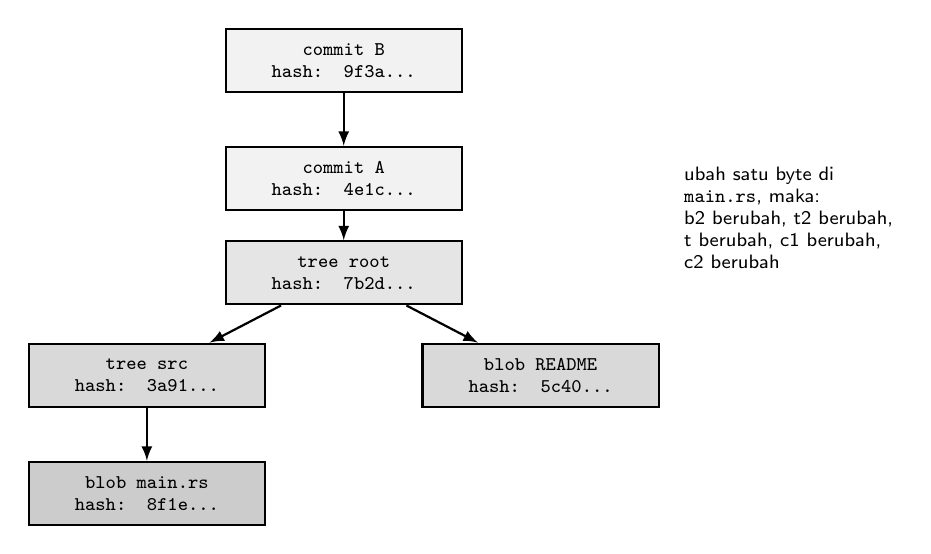
\begin{tikzpicture}[
			node distance=0.6cm and 1.2cm,
			nodebox/.style={rectangle, draw=black, thick, minimum width=3cm, minimum height=0.8cm, align=center, font=\ttfamily\scriptsize},
			line/.style={draw, thick, -latex}
		]
		\node[nodebox, fill=black!5] (c2) at (0, 3.5) {commit B \\ hash: 9f3a...};
		\node[nodebox, fill=black!5] (c1) at (0, 2.0) {commit A \\ hash: 4e1c...};
		\node[nodebox, fill=black!10] (t) at (0, 0.8) {tree root \\ hash: 7b2d...};
		\node[nodebox, fill=black!15] (t2) at (-2.5, -0.5) {tree src \\ hash: 3a91...};
		\node[nodebox, fill=black!15] (b1) at (2.5, -0.5) {blob README \\ hash: 5c40...};
		\node[nodebox, fill=black!20] (b2) at (-2.5, -2.0) {blob main.rs \\ hash: 8f1e...};

		\draw[line] (c2) -- (c1);
		\draw[line] (c1) -- (t);
		\draw[line] (t) -- (t2);
		\draw[line] (t) -- (b1);
		\draw[line] (t2) -- (b2);

		\node[font=\scriptsize\sffamily, anchor=west, align=left] at (4.2, 1.5) {ubah satu byte di\\\texttt{main.rs}, maka:\\b2 berubah, t2 berubah,\\t berubah, c1 berubah,\\c2 berubah};
	\end{tikzpicture}
	\caption{Pohon Merkle pada object store. Perubahan pada satu blob merambat sampai ke commit teratas.}
	\label{fig:merkle}
\end{figure}

\subsection{Mengapa Immutability Terjadi dengan Sendirinya}

Immutability bukan fitur yang ditambahkan ke sistem; ia adalah konsekuensi langsung dari alamat berbasis hash. Jika objek dengan alamat \texttt{H} bisa diubah isinya, maka hash dari isi yang baru tidak akan sama dengan \texttt{H}, dan alamat itu tidak lagi merujuk objek tersebut. Dengan kata lain, "mengubah objek" berarti "membuat objek baru dengan alamat baru"; objek lama tetap ada dengan alamat lamanya.

Sifat ini membawa tiga konsekuensi praktis. Pertama, riwayat tidak bisa ditulis ulang tanpa mengubah semua hash setelah titik perubahan. Kedua, dua pengguna yang memiliki hash yang sama bisa yakin bahwa mereka memiliki isi yang sama. Ketiga, commit bisa di-verifikasi secara offline; pembaca tidak perlu server untuk memastikan bahwa commit yang ia terima benar-benar berasal dari penulis yang diklaim.

Gambar~\ref{fig:immutability} menyandingkan sifat mutable dan immutable pada sistem penyimpanan.

\begin{figure}[H]
	\centering
	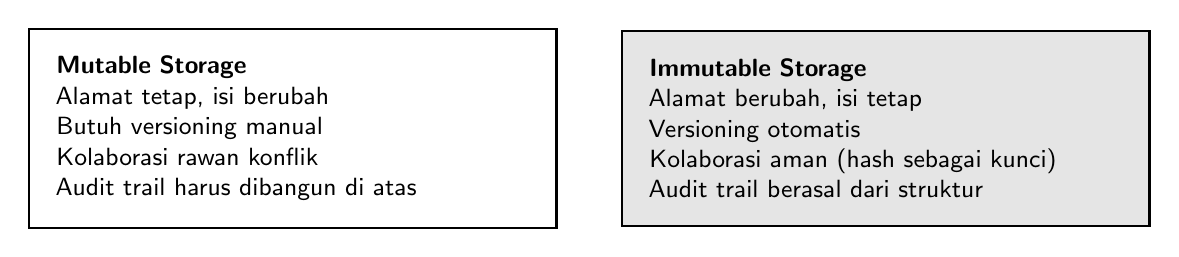
\begin{tikzpicture}[
			box/.style={rectangle, draw=black, thick, text width=6cm, align=left, font=\sffamily\small, inner sep=10pt}
		]
		\node[box, fill=white] (a) {
			\textbf{Mutable Storage} \\
			Alamat tetap, isi berubah \\
			Butuh versioning manual \\
			Kolaborasi rawan konflik \\
			Audit trail harus dibangun di atas
		};
		\node[box, fill=black!10, right=0.8cm of a] (b) {
			\textbf{Immutable Storage} \\
			Alamat berubah, isi tetap \\
			Versioning otomatis \\
			Kolaborasi aman (hash sebagai kunci) \\
			Audit trail berasal dari struktur
		};
	\end{tikzpicture}
	\caption{Perbandingan mutable dan immutable storage.}
	\label{fig:immutability}
\end{figure}

\subsection{Siklus Hidup Satu Objek}

Proses penyimpanan satu objek pada content-addressable storage mengikuti lima langkah yang tetap. Gambar~\ref{fig:store-cycle} menunjukkan siklusnya.

\begin{figure}[H]
	\centering
	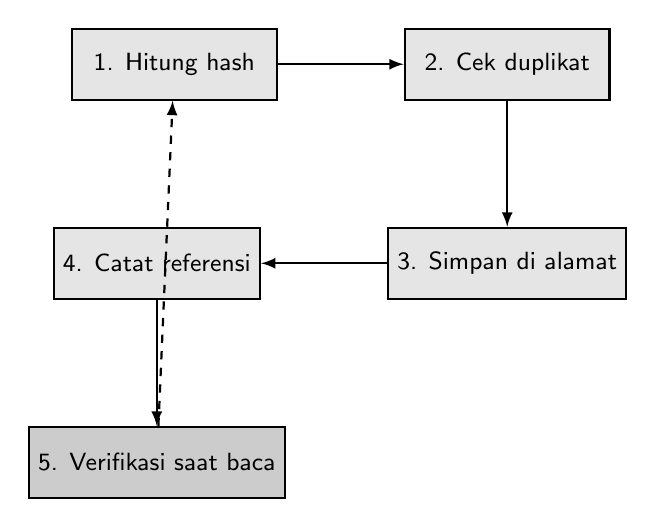
\begin{tikzpicture}[
			node distance=1.6cm,
			box/.style={rectangle, draw=black, thick, fill=black!10, minimum width=2.6cm, minimum height=0.9cm, align=center, font=\sffamily\small},
			line/.style={draw, thick, -latex}
		]
		\node[box] (hash) {1. Hitung hash};
		\node[box, right=of hash] (check) {2. Cek duplikat};
		\node[box, below=of check] (store) {3. Simpan di alamat};
		\node[box, left=of store] (index) {4. Catat referensi};
		\node[box, below=of index, fill=black!20] (verify) {5. Verifikasi saat baca};

		\draw[line] (hash) -- (check);
		\draw[line] (check) -- (store);
		\draw[line] (store) -- (index);
		\draw[line] (index) -- (verify);
		\draw[line, dashed] (verify) -- (hash);
	\end{tikzpicture}
	\caption{Siklus lima tahap penyimpanan objek pada content-addressable storage.}
	\label{fig:store-cycle}
\end{figure}

Garis putus-putus dari verifikasi kembali ke hash menandakan bahwa pembacaan objek berikutnya akan mengulang siklus yang sama. Verifikasi integritas tidak terjadi sekali; ia terjadi setiap kali objek dibaca.

\section{Perbandingan Model Penyimpanan}

Setelah memahami hash, empat tipe objek, dan struktur Merkle, perbedaan antara content-addressable storage dan address-based storage dapat diringkas dalam satu tabel. Tabel~\ref{tab:storage-comparison} menyandingkannya pada tujuh aspek.

\begin{table}[H]
	\centering
	\caption{Perbandingan address-based dan content-addressable storage.}
	\label{tab:storage-comparison}
	\footnotesize
	\begin{tabularx}{\textwidth}{l X X}
		\toprule
		Aspek                     & Address-Based                         & Content-Addressable                \\
		\midrule
		Alamat                    & nomor inode, path, offset             & hash dari isi                      \\
		Duplikasi                 & setiap file adalah salinan baru       & hanya satu salinan per isi unik    \\
		Integritas                & tidak terdeteksi tanpa tool eksternal & terdeteksi saat baca               \\
		Mutability                & isi berubah tanpa ganti alamat        & isi berubah berarti alamat berubah \\
		Kolaborasi                & butuh mekanisme lock eksternal        & aman karena hash sebagai kunci     \\
		Pemulihan setelah korupsi & dari backup eksternal                 & dari replika lain dengan hash sama \\
		Contoh sistem             & ext4, NTFS, FAT32                     & Git, Mercurial, libvctrl, IPFS     \\
		\bottomrule
	\end{tabularx}
\end{table}

Dua paragraf penutup dari perbandingan ini. Pertama, content-addressable storage bukan pengganti sistem berkas; ia adalah lapisan di atas sistem berkas. Objek disimpan sebagai file biasa dengan nama hash, di dalam direktori biasa. Kedua, model ini memindahkan sebagian besar kerumitan dari kode aplikasi ke struktur penyimpanan itu sendiri. Aplikasi tidak perlu memverifikasi integritas, tidak perlu menangani duplikasi, dan tidak perlu menulis log audit; semuanya berasal dari struktur alamat.

\section{Studi Kasus: Menyimpan Satu Commit dari Nol}

\subsection{Langkah 1: Tentukan Isi File}

Misalkan sebuah proyek memiliki satu file, \texttt{notes.txt}, dengan isi dua baris. Di content-addressable storage, isi dihitung sebagai byte mentah, bukan sebagai baris.

\begin{lstlisting}[style=code]
printf "hello\nworld\n" > notes.txt
\end{lstlisting}

\subsection{Langkah 2: Hitung Hash Blob}

Isi file dihash. Hasilnya adalah alamat dari \texttt{blob}.

\begin{lstlisting}[style=code]
sha256sum notes.txt
\end{lstlisting}

\begin{lstlisting}[style=out]
8d9e3f4c1b8a7d2e6f5c4b3a2e1d0c9b8a7f6e5d4c3b2a1f0e9d8c7b6a5f4e3d  notes.txt
\end{lstlisting}

Alamat ini adalah identitas dari isi \texttt{notes.txt}, bukan identitas dari file bernama \texttt{notes.txt}. Jika ada file lain bernama \texttt{backup.txt} dengan isi yang sama, keduanya akan memiliki alamat yang sama.

\subsection{Langkah 3: Cek Duplikat Sebelum Menyimpan}

Sebelum menyimpan, sistem memeriksa apakah alamat sudah ada. Jika sudah, tidak ada yang perlu disimpan.

\begin{lstlisting}[style=code]
test -f .git/objects/8d/9e3f4c1b8a7d2e6f5c4b3a2e1d0c9b8a7f6e5d4c3b2a1f0e9d8c7b6a5f4e3d \
  && echo "already exists" \
  || echo "must store"
\end{lstlisting}

\begin{lstlisting}[style=out]
must store
\end{lstlisting}

Pada percobaan pertama, alamat belum ada, sehingga \texttt{blob} disimpan. Pada percobaan berikutnya dengan isi yang sama, alamat sudah ada, dan sistem tidak menyimpan apa pun.

\subsection{Langkah 4: Simpan Blob di Alamat Hash}

Blob disimpan sebagai file dengan nama hash, di dalam direktori dua karakter pertama. Konvensi ini mencegah direktori berisi puluhan ribu file.

\begin{lstlisting}[style=code]
mkdir -p .git/objects/8d
cp notes.txt .git/objects/8d/9e3f4c1b8a7d2e6f5c4b3a2e1d0c9b8a7f6e5d4c3b2a1f0e9d8c7b6a5f4e3d
\end{lstlisting}

Setelah langkah ini, \texttt{blob} sudah ada di object store. Tetapi \texttt{blob} tidak tahu namanya sendiri. Nama \texttt{notes.txt} belum tersimpan di mana pun.

\subsection{Langkah 5: Bangun Tree yang Memetakan Nama ke Blob}

\texttt{tree} adalah daftar entri. Setiap entri mencatat nama, mode, dan hash. Untuk proyek dengan satu file, \texttt{tree} berisi satu entri.

\begin{lstlisting}[style=code]
printf "100644 blob 8d9e3f4c1b8a7d2e6f5c4b3a2e1d0c9b8a7f6e5d4c3b2a1f0e9d8c7b6a5f4e3d\tnotes.txt\n" \
  > /tmp/tree.txt
\end{lstlisting}

Baris ini menyatakan: entri bernama \texttt{notes.txt}, dengan mode \texttt{100644} (file biasa yang tidak bisa dieksekusi), menunjuk ke \texttt{blob} dengan hash yang sudah dihitung di langkah dua.

\subsection{Langkah 6: Hash Tree}

Hash dari isi \texttt{tree} menjadi alamat \texttt{tree}. Langkah ini menghasilkan hash yang mencakup hash semua \texttt{blob} di dalamnya.

\begin{lstlisting}[style=code]
sha256sum /tmp/tree.txt
\end{lstlisting}

\begin{lstlisting}[style=out]
a1b2c3d4e5f60718293a4b5c6d7e8f90a1b2c3d4e5f60718293a4b5c6d7e8f90  /tmp/tree.txt
\end{lstlisting}

Dua properti penting. Pertama, hash ini bukan hash dari \texttt{blob}; ia adalah hash dari daftar entri yang di dalamnya tercantum hash \texttt{blob}. Kedua, jika isi \texttt{tree} diubah urutannya, hash-nya juga berubah; itulah sebabnya \texttt{tree} selalu diurutkan sebelum dihash.

\subsection{Langkah 7: Bangun Commit}

Commit menyimpan hash dari \texttt{tree}, daftar parent (kosong untuk commit pertama), penulis, committer, timestamp, dan pesan.

\begin{lstlisting}[style=code]
{
  printf "tree a1b2c3d4e5f60718293a4b5c6d7e8f90a1b2c3d4e5f60718293a4b5c6d7e8f90\n"
  printf "author Alice <alice@example.com> 1700000000 +0000\n"
  printf "committer Alice <alice@example.com> 1700000000 +0000\n"
  printf "\n"
  printf "first commit\n"
} > /tmp/commit.txt
\end{lstlisting}

\subsection{Langkah 8: Hash Commit dan Update Ref}

Hash dari isi commit menjadi alamat commit. Langkah terakhir adalah menulis alamat ini ke \texttt{refs/heads/main}, sehingga commit bisa ditemukan melalui nama branch.

\begin{lstlisting}[style=code]
sha256sum /tmp/commit.txt
printf "%s\n" "f7e6d5c4b3a2918271a2b3c4d5e6f708a9b0c1d2e3f405162738495a6b7c8d9e" \
  > .git/refs/heads/main
\end{lstlisting}

Setelah langkah ini, seluruh isi commit sudah tersimpan di object store. Untuk membaca kembali \texttt{notes.txt} pada commit tersebut, sistem cukup membaca \texttt{refs/heads/main}, membaca commit di alamat itu, membaca \texttt{tree} di alamat yang tercantum di commit, dan membaca \texttt{blob} di alamat yang tercantum di \texttt{tree}.

\subsection{Ringkasan Studi Kasus}

\begin{table}[H]
	\centering
	\caption{Ringkasan delapan langkah menyimpan satu commit.}
	\label{tab:case-summary}
	\footnotesize
	\begin{tabularx}{\textwidth}{l X X}
		\toprule
		Langkah & Operasi                             & Hasil                                              \\
		\midrule
		1       & tentukan isi file                   & \texttt{notes.txt} dengan dua baris                \\
		2       & hash \texttt{blob}                  & alamat \texttt{blob} (\texttt{8d9e...})            \\
		3       & cek duplikat                        & \texttt{blob} belum ada, harus disimpan            \\
		4       & simpan \texttt{blob}                & file di \texttt{.git/objects/8d/9e...}             \\
		5       & bangun \texttt{tree}                & satu entri (nama, mode, hash)                      \\
		6       & hash \texttt{tree}                  & alamat \texttt{tree} (\texttt{a1b2...})            \\
		7       & bangun \texttt{commit}              & tree + author + committer + pesan                  \\
		8       & hash \texttt{commit} dan update ref & \texttt{refs/heads/main} menunjuk \texttt{f7e6...} \\
		\bottomrule
	\end{tabularx}
\end{table}

\section{Kesalahan Umum dan Cara Menghindarinya}

\begin{table}[H]
	\centering
	\caption{Kesalahan umum pada implementasi content-addressable storage.}
	\label{tab:mistakes}
	\footnotesize
	\begin{tabularx}{\textwidth}{l X X}
		\toprule
		Kesalahan                               & Akibat                             & Perbaikan                                    \\
		\midrule
		hash tanpa encoding yang konsisten      & hash berbeda untuk isi sama        & tentukan encoding sebelum hash               \\
		cek duplikat dihilangkan                & storage membengkak                 & periksa alamat sebelum menulis               \\
		\texttt{tree} tidak diurutkan           & hash berbeda untuk isi sama        & urutkan entri sebelum hash                   \\
		\texttt{commit} tanpa parent            & semua commit menjadi orphan        & sertakan hash parent                         \\
		\texttt{ref} ditulis langsung ke target & ref korup jika write terputus      & tulis ke temp lalu rename atomik             \\
		\texttt{blob} disimpan tanpa hash       & tidak bisa ditemukan kembali       & hitung hash dulu, baru simpan                \\
		hash disimpan sebagai string hex        & storage lebih besar, lookup lambat & simpan sebagai byte biner                    \\
		pesan commit tanpa newline              & parser gagal                       & tambahkan \texttt{\textbackslash n} di akhir \\
		timestamp lokal bukan UTC               & riwayat tidak konsisten            & simpan dalam UTC                             \\
		hapus \texttt{blob} yang masih dirujuk  & commit lama menjadi korup          & gunakan ref-count atau GC                    \\
		\bottomrule
	\end{tabularx}
\end{table}

Dua kesalahan yang paling sering muncul adalah tidak mengurutkan entri \texttt{tree} sebelum hash dan menyimpan hash sebagai string hex. Yang pertama membuat dua \texttt{tree} dengan isi sama tetapi urutan berbeda memiliki hash yang berbeda, sehingga deduplikasi gagal. Yang kedua membuat setiap lookup dan perbandingan memakan empat kali lipat ruang; untuk dua puluh juta objek, selisih ini menjadi ratusan megabyte.

\section{Lembar Rujukan Cepat}

\begin{table}[H]
	\centering
	\caption{Rujukan cepat perintah dan operasi pada content-addressable storage.}
	\label{tab:quick-reference}
	\footnotesize
	\begin{tabularx}{\textwidth}{l X}
		\toprule
		Kebutuhan                               & Perintah atau operasi                            \\
		\midrule
		hash file                               & \texttt{sha256sum file}                          \\
		hash stdin                              & \texttt{echo -n "x" | sha256sum}                 \\
		verifikasi hash                         & \texttt{sha256sum -c checksum.txt}               \\
		cek \texttt{blob} ada                   & \texttt{test -f .git/objects/ab/cdef...}         \\
		simpan \texttt{blob}                    & \texttt{mkdir -p .git/objects/ab} lalu copy file \\
		baca \texttt{blob}                      & \texttt{cat .git/objects/ab/cdef...}             \\
		baca \texttt{tree}                      & \texttt{git cat-file -p <tree-hash>}             \\
		baca \texttt{commit}                    & \texttt{git cat-file -p <commit-hash>}           \\
		update ref                              & \texttt{git update-ref refs/heads/main <hash>}   \\
		list semua ref                          & \texttt{git show-ref}                            \\
		baca HEAD                               & \texttt{cat .git/HEAD}                           \\
		root \texttt{tree} dari \texttt{commit} & \texttt{git rev-parse <hash>\^{}tree}            \\
		\texttt{tree} dari path                 & \texttt{git ls-tree <tree-hash> path/}           \\
		diff dua \texttt{tree}                  & \texttt{git diff-tree <tree1> <tree2>}           \\
		verifikasi integritas                   & \texttt{git fsck}                                \\
		pack objek                              & \texttt{git gc}                                  \\
		prune unreachable                       & \texttt{git prune}                               \\
		lihat history                           & \texttt{git log --graph --oneline}               \\
		trace perubahan baris                   & \texttt{git blame file}                          \\
		cek hash commit saat ini                & \texttt{git rev-parse HEAD}                      \\
		\bottomrule
	\end{tabularx}
\end{table}

\section{Kesimpulan}

Content-addressable storage adalah model penyimpanan di mana alamat objek ditentukan oleh isinya. Hash kriptografis memastikan bahwa setiap perubahan sekecil apa pun menghasilkan alamat yang berbeda. Empat tipe objek, yaitu \texttt{blob}, \texttt{tree}, \texttt{commit}, dan \texttt{tag}, bekerja sama dalam struktur Merkle di mana hash setiap level mencakup hash level di bawahnya. Immutability bukan fitur tambahan; ia adalah konsekuensi dari alamat berbasis isi.

Tiga prinsip penutup:

\begin{enumerate}
	\item Alamat adalah isi. Jika dua objek harus dianggap sama, mereka harus memiliki alamat yang sama. Jika mereka harus berbeda, alamatnya harus berbeda. Aturan ini menghilangkan hampir semua kerumitan yang biasanya muncul pada sistem deduplikasi manual.
	\item Urutan adalah bagian dari isi. Dua \texttt{tree} dengan entri yang sama tetapi urutan berbeda adalah dua objek yang berbeda. Selalu urutkan sebelum menghitung hash, dan dokumentasikan aturan pengurutannya.
	\item Immutability adalah fondasi, bukan kemewahan. Sistem yang mengizinkan objek berubah tanpa mengganti alamatnya kehilangan semua jaminan yang ditawarkan content-addressable storage: verifikasi integritas, deduplikasi otomatis, dan audit trail yang bisa dipercaya. Jangan pernah menulis ulang objek setelah alamatnya dipublikasikan.
\end{enumerate}

Dengan kerangka ini, pembaca siap membaca implementasi VCS mana pun, atau membangun VCS kecil sendiri di atas model yang sudah terbukti.

\newpage
\section*{Referensi}
\addcontentsline{toc}{section}{Referensi}

\begin{thebibliography}{99}

	\bibitem{chacon}
	Chacon, S., \& Straub, B. (2014).
	\textit{Pro Git} (2nd ed.).
	Apress.
	\texttt{https://git-scm.com/book/}

	\bibitem{loeliger}
	Loeliger, J., \& McCullough, M. (2012).
	\textit{Version Control with Git} (2nd ed.).
	O'Reilly Media.

	\bibitem{git-internals}
	Git Project. (2026).
	\textit{Git Internals --- Git Objects}.
	Git Documentation.
	\texttt{https://git-scm.com/book/en/v2/Git-Internals-Git-Objects}

	\bibitem{merkle}
	Merkle, R. C. (1988).
	A Digital Signature Based on a Conventional Encryption Function.
	In \textit{Advances in Cryptology --- CRYPTO '87}
	(pp. 369--378). Springer.

	\bibitem{nist-sha}
	NIST. (2015).
	\textit{Secure Hash Standard (SHS)} (FIPS PUB 180-4).
	National Institute of Standards and Technology.
	\texttt{https://doi.org/10.6028/NIST.FIPS.180-4}

	\bibitem{rfc6234}
	Eastlake, D., \& Hansen, T. (2011).
	\textit{US Secure Hash Algorithms (SHA and SHA-based HMAC and HKDF)} (RFC 6234). IETF.

	\bibitem{libvctrl}
	Khafidi, M. R. (2026).
	\textit{libvctrl: A Precision Toolkit for Building Custom Version Control Systems}.
	GitHub.
	\texttt{https://github.com/mroczect/libvctrl}

\end{thebibliography}

\end{document}
